% Options for packages loaded elsewhere
\PassOptionsToPackage{unicode}{hyperref}
\PassOptionsToPackage{hyphens}{url}
\PassOptionsToPackage{dvipsnames,svgnames,x11names}{xcolor}
%
\documentclass[
]{article}
\usepackage{amsmath,amssymb}
\usepackage{fancyvrb}
\usepackage{fvextra}
%\RecustomVerbatimEnvironment{verbatim}{Verbatim}{commandchars=\\\{\}}
\usepackage{lmodern}
\usepackage{bold-extra}
\usepackage{iftex}
\ifPDFTeX
  \usepackage[T1]{fontenc}
  \usepackage[utf8]{inputenc}
  \usepackage{textcomp} % provide euro and other symbols
\else % if luatex or xetex
  \usepackage{unicode-math}
  \defaultfontfeatures{Scale=MatchLowercase}
  \defaultfontfeatures[\rmfamily]{Ligatures=TeX,Scale=1}
\fi
% Use upquote if available, for straight quotes in verbatim environments
\IfFileExists{upquote.sty}{\usepackage{upquote}}{}
\IfFileExists{microtype.sty}{% use microtype if available
  \usepackage[]{microtype}
  \UseMicrotypeSet[protrusion]{basicmath} % disable protrusion for tt fonts
}{}
\makeatletter
\@ifundefined{KOMAClassName}{% if non-KOMA class
  \IfFileExists{parskip.sty}{%
    \usepackage{parskip}
  }{% else
    \setlength{\parindent}{0pt}
    \setlength{\parskip}{6pt plus 2pt minus 1pt}}
}{% if KOMA class
  \KOMAoptions{parskip=half}}
\makeatother
\usepackage{xcolor}
\usepackage{graphicx}
\makeatletter
\def\maxwidth{\ifdim\Gin@nat@width>\linewidth\linewidth\else\Gin@nat@width\fi}
\def\maxheight{\ifdim\Gin@nat@height>\textheight\textheight\else\Gin@nat@height\fi}
\makeatother
% Scale images if necessary, so that they will not overflow the page
% margins by default, and it is still possible to overwrite the defaults
% using explicit options in \includegraphics[width, height, ...]{}
\setkeys{Gin}{width=\maxwidth,height=\maxheight,keepaspectratio}
% Set default figure placement to htbp
\makeatletter
\def\fps@figure{htbp}
\makeatother
\setlength{\emergencystretch}{3em} % prevent overfull lines
\providecommand{\tightlist}{%
  \setlength{\itemsep}{0pt}\setlength{\parskip}{0pt}}
\setcounter{secnumdepth}{5}
\newlength{\cslhangindent}
\setlength{\cslhangindent}{1.5em}
\newlength{\csllabelwidth}
\setlength{\csllabelwidth}{3em}
\newlength{\cslentryspacingunit} % times entry-spacing
\setlength{\cslentryspacingunit}{\parskip}
\newenvironment{CSLReferences}[2] % #1 hanging-ident, #2 entry spacing
 {% don't indent paragraphs
  \setlength{\parindent}{0pt}
  % turn on hanging indent if param 1 is 1
  \ifodd #1
  \let\oldpar\par
  \def\par{\hangindent=\cslhangindent\oldpar}
  \fi
  % set entry spacing
  \setlength{\parskip}{\cslentryspacingunit}
 }%
 {}
\usepackage{calc}
\newcommand{\CSLBlock}[1]{#1\hfill\break}
\newcommand{\CSLLeftMargin}[1]{\parbox[t]{\csllabelwidth}{#1}}
\newcommand{\CSLRightInline}[1]{\parbox[t]{\linewidth - \csllabelwidth}{#1}\break}
\newcommand{\CSLIndent}[1]{\hspace{\cslhangindent}#1}
\makeatletter
\@ifpackageloaded{subfig}{}{\usepackage{subfig}}
\@ifpackageloaded{caption}{}{\usepackage{caption}}
\captionsetup[subfloat]{margin=0.5em}
\AtBeginDocument{%
\renewcommand*\figurename{Figure}
\renewcommand*\tablename{Table}
}
\AtBeginDocument{%
\renewcommand*\listfigurename{List of Figures}
\renewcommand*\listtablename{List of Tables}
}
\newcounter{pandoccrossref@subfigures@footnote@counter}
\newenvironment{pandoccrossrefsubfigures}{%
\setcounter{pandoccrossref@subfigures@footnote@counter}{0}
\begin{figure}\centering%
\gdef\global@pandoccrossref@subfigures@footnotes{}%
\DeclareRobustCommand{\footnote}[1]{\footnotemark%
\stepcounter{pandoccrossref@subfigures@footnote@counter}%
\ifx\global@pandoccrossref@subfigures@footnotes\empty%
\gdef\global@pandoccrossref@subfigures@footnotes{{##1}}%
\else%
\g@addto@macro\global@pandoccrossref@subfigures@footnotes{, {##1}}%
\fi}}%
{\end{figure}%
\addtocounter{footnote}{-\value{pandoccrossref@subfigures@footnote@counter}}
\@for\f:=\global@pandoccrossref@subfigures@footnotes\do{\stepcounter{footnote}\footnotetext{\f}}%
\gdef\global@pandoccrossref@subfigures@footnotes{}}
\@ifpackageloaded{float}{}{\usepackage{float}}
\floatstyle{ruled}
\@ifundefined{c@chapter}{\newfloat{codelisting}{h}{lop}}{\newfloat{codelisting}{h}{lop}[chapter]}
\floatname{codelisting}{Listing}
\newcommand*\listoflistings{\listof{codelisting}{List of Listings}}
\makeatother
\ifLuaTeX
  \usepackage{selnolig}  % disable illegal ligatures
\fi
\IfFileExists{bookmark.sty}{\usepackage{bookmark}}{\usepackage{hyperref}}
\IfFileExists{xurl.sty}{\usepackage{xurl}}{} % add URL line breaks if available
\urlstyle{same} % disable monospaced font for URLs
\hypersetup{
  pdftitle={Notes on Color},
  pdfauthor={Tyler Neylon},
  colorlinks=true,
  linkcolor={black},
  filecolor={Maroon},
  citecolor={Blue},
  urlcolor={Blue},
  pdfcreator={LaTeX via pandoc}}

\title{Notes on Color}
\author{Tyler Neylon}
\date{\href{https://tylerneylon.com/a/7date/}{352.2024}}

%%%%%%%%%%%%%%%%%%%%%%%%%%%%%%%%%%%%%%%%%%%%%%%%%%%%%%%%%%%%%%%%%%%%%%%%%%%
% Begin custom, non-pandoc commands.

\newcommand{\customstrut}{\rule[-3mm]{0mm}{7.5mm}}
\newenvironment{densearray}{\begin{array}{rcl}}{\end{array}}
\newcommand{\class}[1]{}
\newcommand{\Rule}[3]{}
\newcommand{\optquad}{\quad}
\newcommand{\smallscrneg}{}
\newcommand{\smallscr}[1]{}
\newcommand{\bigscr}[1]{#1}
\newcommand{\smallscrskip}[1]{}

% I learned some things from these two links:
% https://tex.stackexchange.com/questions/145812/using-fbox-in-a-newenvironment
% https://tex.stackexchange.com/questions/120042/splitting-a-command-syntax-across-a-newenvironment-definition

\newsavebox{\mybox}
\newenvironment{myboxed}{\begin{lrbox}{\mybox}\begin{minipage}{0.98\textwidth}}{\end{minipage}\end{lrbox}\fbox{\usebox{\mybox}}}

\newcommand{\boxedstart}{\begin{myboxed}}
\newcommand{\boxedend}{\end{myboxed}}

\newcommand{\crossedouty}{\dot y \kern -4.5pt \raise 4.9pt \hbox{\(\scriptscriptstyle\diagup\)}}
\newcommand{\crossedoutone}{\dot 1 \kern -5.1pt \raise 6.6pt \hbox{\(\scriptscriptstyle\diagup\)}}
\newcommand{\crossedouttwo}{\dot 2 \kern -5.1pt \raise 6.6pt \hbox{\(\scriptscriptstyle\diagup\)}}
\newcommand{\crossedoutthree}{\dot 3 \kern -5.1pt \raise 6.6pt \hbox{\(\scriptscriptstyle\diagup\)}}
\newcommand{\crossedoutfive}{\dot 5 \kern -5.1pt \raise 6.6pt \hbox{\(\scriptscriptstyle\diagup\)}}
\newcommand{\crossedoutsix}{\dot 6 \kern -5.1pt \raise 6.6pt \hbox{\(\scriptscriptstyle\diagup\)}}
\newcommand{\crossedoutseven}{\dot 7 \kern -5.1pt \raise 6.6pt \hbox{\(\scriptscriptstyle\diagup\)}}
\newcommand{\lowerhaty}{\lower 1ex\hbox{\(\hat y\)}}
\newcommand{\lhy}{\lower 1ex\hbox{\(\hat y\)}}

\let\smallstart\iffalse
\let\smallend\fi

% End custom, non-pandoc commands.
%%%%%%%%%%%%%%%%%%%%%%%%%%%%%%%%%%%%%%%%%%%%%%%%%%%%%%%%%%%%%%%%%%%%%%%%%%%

\begin{document}
\maketitle

\newcommand{\R}{\mathbb{R}}
\newcommand{\N}{\mathbb{N}}
\newcommand{\eqnset}[1]{\left.\mbox{$#1$}\;\;\right\rbrace\class{postbrace}{ }}
\providecommand{\latexonlyrule}[3][]{}
\providecommand{\optquad}{\class{optquad}{}}
\providecommand{\smallscrneg}{\class{smallscrneg}{ }}
\providecommand{\bigscr}[1]{\class{bigscr}{#1}}
\providecommand{\smallscr}[1]{\class{smallscr}{#1}}
\providecommand{\smallscrskip}[1]{\class{smallscrskip}{\hskip #1}}

\newcommand{\mydots}{{\cdot}\kern -0.1pt{\cdot}\kern -0.1pt{\cdot}}

\newcommand{\?}{\stackrel{?}{=}}
\newcommand{\sign}{\textsf{sign}}
\newcommand{\order}{\textsf{order}}
\newcommand{\flips}{\textsf{flips}}
\newcommand{\samecycles}{\textsf{same$\\\_$cycles}}
\newcommand{\canon}{\textsf{canon}}
\newcommand{\cs}{\mathsf{cs}}
\newcommand{\dist}{\mathsf{dist}}
\renewcommand{\theenumi}{(\roman{enumi})}

{[} Formats:
\href{http://tylerneylon.com/a/color_notes/color_notes.html}{html}
\textbar{}
\href{http://tylerneylon.com/a/color_notes/color_notes.pdf}{pdf}
\(\,\){]}

This post captures my own notes about color, categorized according to
some key questions I had when I began.

I have a daydream of one day writing up something like an engineer's
guide to color that is at once engaging, well-designed, educational, and
a pleasure to read. For now I'm just aiming for educational.

\hypertarget{questions-about-light-and-color-itself}{%
\section{Questions about light and color
itself}\label{questions-about-light-and-color-itself}}

\begin{itemize}
\tightlist
\item
  What is color, physically?
\item
  How do blacklights work?
\item
  How does infrared light interact with heat?
\end{itemize}

\hypertarget{the-nature-of-human-vision}{%
\section{The nature of human vision}\label{the-nature-of-human-vision}}

\hypertarget{how-do-we-know-human-color-vision-is-3-dimensional}{%
\subsection{How do we know human color vision is
3-dimensional?}\label{how-do-we-know-human-color-vision-is-3-dimensional}}

There are two main pieces of evidence that human color vision is
3-dimensional. One is a classic color-matching experiment, and the other
is based on human retinal anatomy --- the fact that we have three types
of cones in our retinas.

\hypertarget{color-matching-experiments}{%
\subsubsection{Color-matching
experiments}\label{color-matching-experiments}}

Here's the setup for the classic color-matching experiment: A human sits
staring at a wall in a dark room. They see a circle of colored light.
The light on the left side is a single pure wavelength --- this is
called a \emph{spectral color}. The light on the right hand side is a
weighted combination of three primary colors (colors of fixed, known
wavelengths).

The poor human is tasked with adjusting the intensities of the three
primaries in order to make the right-hand side match the color of the
left-hand side.

One thing to note is that, if humans were completely color-blind, and
only saw in black and white, then this experiment could succeed with
only a single primary color. In fact, you can do this experiment with a
single primary color in extremely low light, and indeed you can match
any color in that setting (TODO REFERENCE). The fact that this
experiment succeeds --- that you can always find a perfect match ---
with three primary colors is a huge piece of evidence that our color
vision is fundamentally 3-dimensional. I am a very skeptical person, so
I will point out that the traditional experiments did not perform a
systematic investigation of different intensities of the target color,
and I would prefer to see that kind of investigation before fully
agreeing that human color vision is three-dimensional.

I have slightly simplified my explanation of the color-matching
experiment above, and now I'll come clean and try to provide the detail
I had left out. If the experiment above worked exactly as I described,
then for every wavelength (of the target color on the left), you'd have
three non-negative coefficients for the primary colors on the right.
Those coefficients would describe quantitatively how the target color is
capture by the primary colors.

However, there are some cases where a match is not possible in the
traditional way; but there's an easy fix. Suppose your target color is
some kind of teal color, and you're mixing green and blue on the right,
but the right side always looks a little more yellow-ish than the right
side. Well, if you add a little red to the \emph{left} side (which would
move it toward yellow), then you can achieve a match. This actually
happens. But the matches are still always possible. The result is that
we allow for \emph{negative} coefficients in the color matching data.

You might naturally ask: Why can't we just choose the right primary
colors so that we never need negative coefficients? And it turns out
that's impossible, as I'll explain below.\footnote{As a spoiler that
  might not make sense yet but will later: It turns out that the
  geometry of spectral colors is a shape that is never the convex hull
  of three points. For any three primary colors you choose, you can use
  non-negative combinations of those colors to represent any color in
  the triangle between them (inside their convex hull). But there will
  always be spectral colors outside this triangle.} But the experiment
still shows that there's always a linear dependency between any
wavelength and the primary colors of the experiment. If we write the
target color as a vector \(T\), and the primary colors as \(R, G, B\),
then we can always find coefficients (possibly negative) to satisfy this
equation:

\[T = a R + b G + c B.\]

The argument goes: If we had obviously 4-dimensional color perception,
then there would be some target color \(T\) such that no values of
\(a,b,c\) could match it, just as no combination of red and green can
match blue. By the way, I've chosen the somewhat-awkward variables
\(a,b,c\) (awkward since you might think \(b\) matches ``blue,'' but it
doesn't) because this researcher named John Guild published pivotal
color vision data about such an experiment in 1931, which (along with
other work), led to the creation of the famous chromaticity diagram that
I'll describe below.

I transcribed the original data from Guild's 1931 paper --- his Table II
--- and re-plotted his RGB coefficients below (Guild 1931).

\begin{figure}
\centering
\begin{center}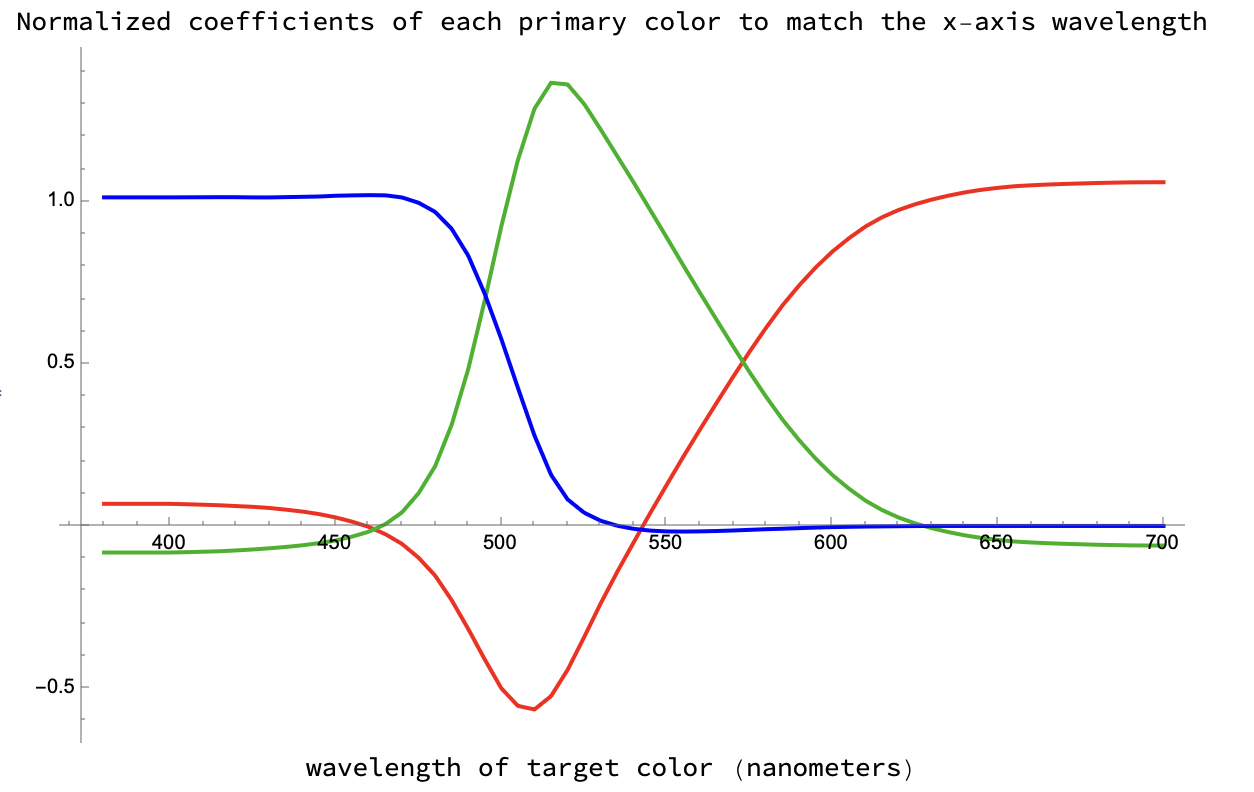
\includegraphics[width=1.0\textwidth]{img/color_matching_coeffs.png}\end{center}
\caption{John Guild's original 1931 color-matching data. Each vertical
line through this graph provides three values that add up to 1; the
coefficients have been normalized (scaled together per x-value) to
ensure this. As a reminder, low wavelengths (near 400nm) indicate blue
shades, and high values (near 700nm) indicate red shades, with the full
spectrum between. Related files:
\href{color_matching/plot_color_matching_coeffs.htm}{Mathematica code to
make this image} \textbar{}
\href{color_matching/plot_color_matching_coeffs.nb}{Mathematica
notebook} \textbar{}
\href{color_matching/guild_color_matching_data.math}{text data from
Guild's Table II}.}
\end{figure}

To arrive at this data, Guild worked with seven (yes, a small number!)
of test subjects (aka people), and averaged their numbers together. One
thing he found is that there is not much variance between
(non-color-blind) people. In the 1931 paper, he referred to his primary
colors as the ``working primaries'' to differentiate them from nearby
colors that were considered ``standard'' at the time. As far as I can
tell, Guild did not directly describe the wavelenghts of his working
primary colors, but did describe how to convert those to standard
primary colors. (TODO THINK ABOUT THIS MORE)

If you're like me, you might be thinking that we're close to seeing cone
sensitivities. But the transformation from this graph to cone
sensitivities is not simple because each cone has a non-linear
sensitivity to a entire range of wavelengths --- more on that below.

In case you're curious about the variance across different people,
here's Guild's original figure showing the same curve for all seven of
his subjects:

\begin{figure}
\centering
\begin{center}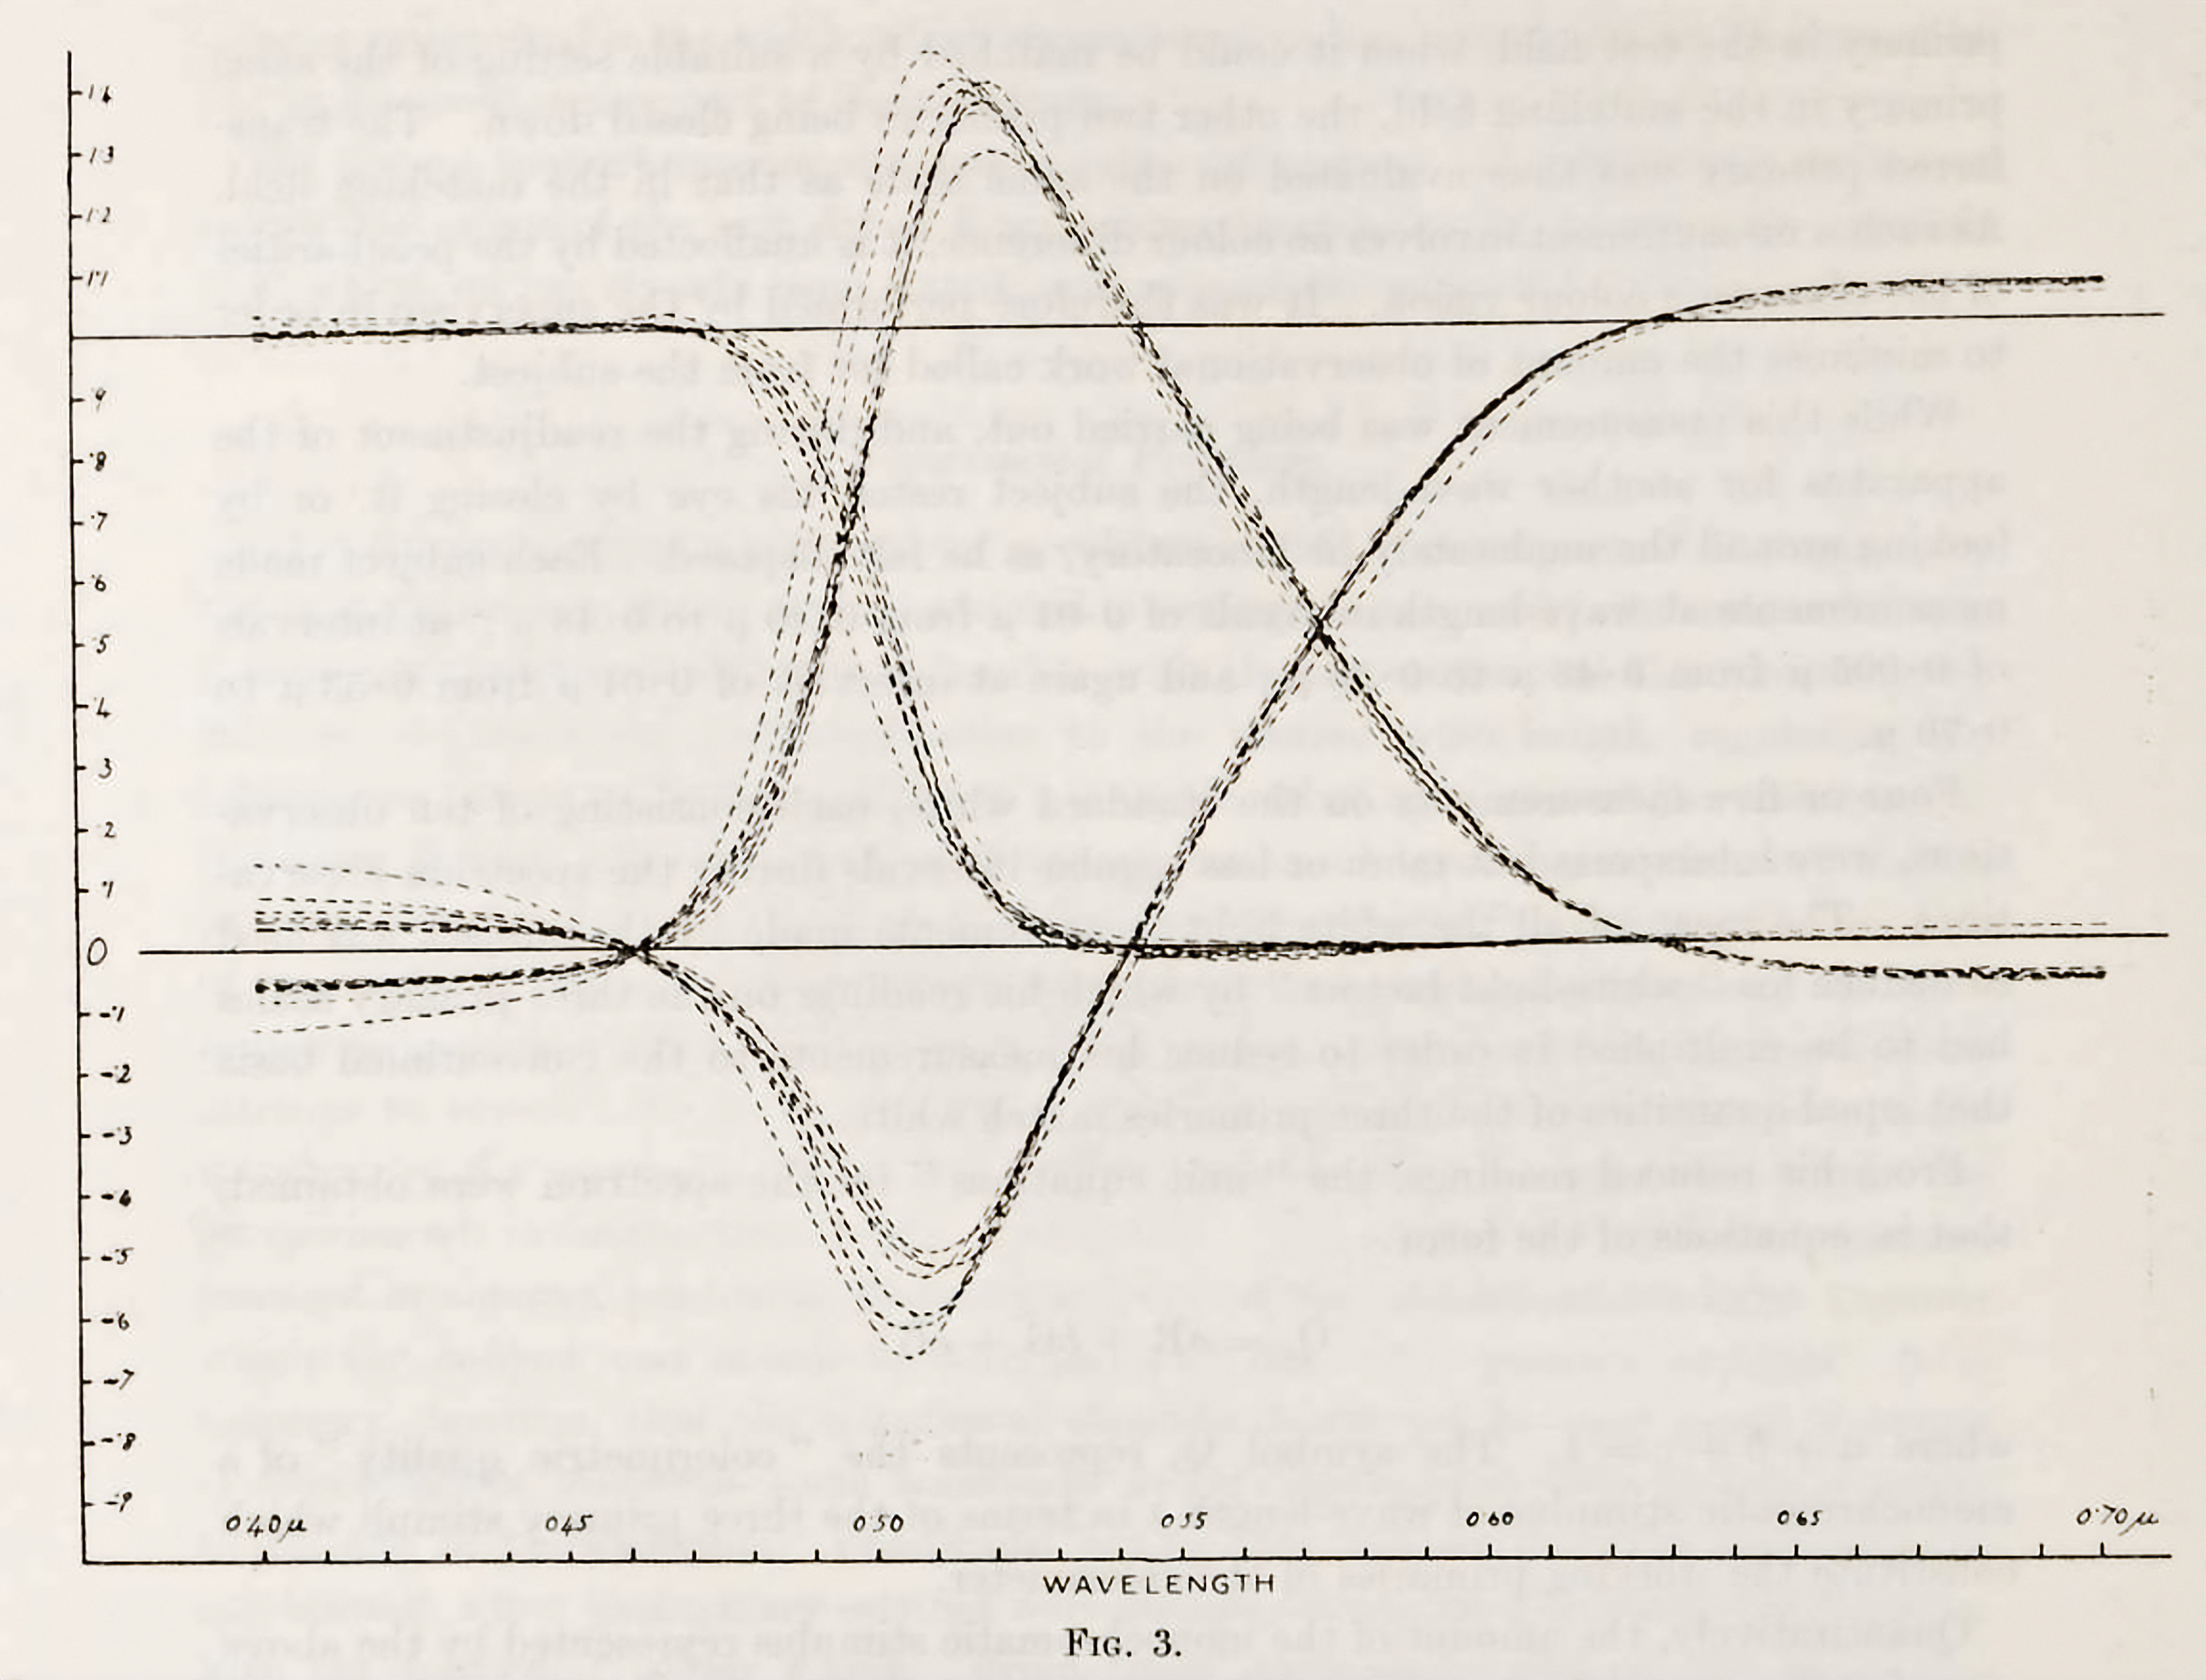
\includegraphics[width=1.0\textwidth]{img/Guild_different_subjects.jpg}\end{center}
\caption{Guild's original diagram showing the similar results from
color-matching experiments across seven subjects. (Guild 1931)}
\end{figure}

As you can see, the curves are fairly consistent, except perhaps for the
extremes of the middle-wavelength primary (green-ish primary, top of
figure) the bottom of the long-wavelength primary (red-ish primary,
bottom of figure). I also see more variation in the red/green portions
on the lower-left, as opposed to the high consistency in the blue
saturation (top-left) and in all primary coefficients on the right of
the figure.

\hypertarget{we-have-three-kinds-of-cones}{%
\subsubsection{We have three kinds of
cones}\label{we-have-three-kinds-of-cones}}

HERE

\hypertarget{if-we-have-three-kinds-of-cones-and-also-rods-why-dont-we-have-4-dimensional-color-vision}{%
\section{If we have three kinds of cones and also rods, why don't we
have 4-dimensional color
vision?}\label{if-we-have-three-kinds-of-cones-and-also-rods-why-dont-we-have-4-dimensional-color-vision}}

AND HERE NEXT

\begin{itemize}
\tightlist
\item
  How do we know that color is a 3-dimensional thing?

  \begin{itemize}
  \tightlist
  \item
    Related: If we have 3 types of cones plus rods, why isn't color
    4-dimensional?
  \end{itemize}
\item
  Why are red, green, and blue special?
\item
  How do we know humans have 3 types of cones?
\item
  How do rods and cones perceive color?

  \begin{itemize}
  \tightlist
  \item
    Related: What is a mathematical model for how light in the world is
    translated into signals in the brain?
  \end{itemize}
\item
  How do we know the actual cone sensitivies?
\item
  Why do the ends of the rainbow meet up so nicely?

  \begin{itemize}
  \tightlist
  \item
    Related: Are all the colors we see based on physically real colors?
  \end{itemize}
\item
  Why do we see the light spectrum that we do?
\item
  Why is the chromaticity diagram the shape that it is?
\item
  Why do we always need to allow for negative coefficients in color
  matching?
\item
  Are there colors we could theoretically perceive, but can't exist in
  reality?
\item
  How can I model, with mathematical precision, the common types of
  color blindness?
\end{itemize}

\hypertarget{reproducing-colors}{%
\section{Reproducing colors}\label{reproducing-colors}}

\begin{itemize}
\tightlist
\item
  How do monitors and printers reproduce any color?
\item
  Why can't a monitor display all possible colors?
\item
  What are color spaces?
\item
  What are the HSL and HSV color spaces, and how do they differ?
\item
  What's the difference between chroma and saturation?
\item
  What are the formulas for switching between RGB, HSL, and HSV?
\item
  What does the name sRGB indicate?
\end{itemize}

\begin{center}\rule{0.5\linewidth}{0.5pt}\end{center}

\hypertarget{bibliography}{%
\section*{Bibliography}\label{bibliography}}
\addcontentsline{toc}{section}{Bibliography}

\hypertarget{refs}{}
\begin{CSLReferences}{1}{0}
\leavevmode\vadjust pre{\hypertarget{ref-guild1931colorimetric}{}}%
Guild, John. 1931. {``The Colorimetric Properties of the Spectrum.''}
\emph{Philosophical Transactions of the Royal Society of London. Series
A, Containing Papers of a Mathematical or Physical Character} 230
(681-693): 149--87.

\end{CSLReferences}

\end{document}

